\documentclass[aspectratio=169,10pt]{beamer}

\usepackage[utf8]{inputenc}
\usepackage[T1]{fontenc}
\usepackage{lmodern}
\usepackage{textcomp}
\usepackage{booktabs}
\usepackage{tabularx}
\usepackage{tcolorbox}
\usepackage{tikz}
\usepackage{amsmath}
\graphicspath{{./}{figures/}{logos/}{../../figures/}{../../logos/}}

% ------------------------------------------------------------------
% Sober & Visual Theme
% ------------------------------------------------------------------
\definecolor{navy}{RGB}{20,60,115}
\definecolor{navylight}{RGB}{235,242,250}
\definecolor{accent}{RGB}{196,78,82}
\definecolor{accentlight}{RGB}{252,238,238}
\definecolor{okgreen}{RGB}{45,130,80}
\definecolor{oklight}{RGB}{235,247,240}
\definecolor{darkgray}{RGB}{65,65,65}

\setbeamertemplate{navigation symbols}{}
\setbeamercolor{normal text}{fg=darkgray}
\setbeamercolor{frametitle}{fg=navy,bg=white}
\setbeamercolor{title}{fg=navy}
\setbeamercolor{subtitle}{fg=darkgray}
\setbeamercolor{structure}{fg=navy}
\setbeamerfont{frametitle}{size=\Large,series=\bfseries}
\setbeamertemplate{frametitle}{%
  \vspace{5pt}\insertframetitle\par\vspace{-3pt}%
  {\color{accent}\rule{2.2cm}{1.6pt}}\vspace{-2pt}%
}
\setbeamertemplate{itemize items}{\color{accent}$\blacktriangleright$}
\setbeamertemplate{footline}{%
  \hspace{12pt}{\scriptsize\color{gray}Tasko --- Growth Modeling \& Data-Driven Strategy (Groupe 15)}%
  \hfill{\scriptsize\color{gray}\insertframenumber\,/\,\inserttotalframenumber}\hspace{12pt}\vspace{5pt}%
}

\newcommand{\eur}{\,\texteuro}
\newcommand{\pc}{\,\%}
\newcommand{\figtitle}[1]{{\small\bfseries\color{navy}#1}\\[2pt]}

% Highlight card macro: \kpicard{bordercolor}{bgcolor}{bigtext}{subtext}
\newcommand{\kpicard}[4]{%
  \begin{tcolorbox}[colback=#2,colframe=#1,boxrule=0.8pt,arc=3pt,left=4pt,right=4pt,top=5pt,bottom=5pt,width=\linewidth,halign=center]
    {\LARGE\bfseries\color{#1}#3}\\[3pt]
    {\scriptsize\color{darkgray}#4}
  \end{tcolorbox}%
}

% Bottom takeaway bar
\newcommand{\takeaway}[1]{%
  \vspace{2pt}
  \begin{tcolorbox}[colback=navylight,colframe=navy,boxrule=0.5pt,arc=2pt,left=6pt,right=6pt,top=3pt,bottom=3pt]
    \centering\footnotesize\color{navy}\textbf{Key takeaway:} #1
  \end{tcolorbox}%
}

\title{\textbf{Tasko: What Really Drives Growth Before the Series A?}}
\subtitle{Growth Modeling \& Data-Driven Strategy}
\author{\textbf{Groupe 15} \\[4pt] Joe \textsc{El-Hajj} \quad$\cdot$\quad Colomban \textsc{Boisseau} \quad$\cdot$\quad Mouad \textsc{Chouki} \quad$\cdot$\quad Maxime \textsc{Philippon}}
\institute{IMT Atlantique}
\date{2026 -- 2027}

\begin{document}

% ==================================================================
% SLIDE 1: TITLE PAGE
% ==================================================================
\begin{frame}[plain]
  \begin{tikzpicture}[remember picture, overlay]
    \node[anchor=north east, xshift=-0.4cm, yshift=-0.25cm] at (current page.north east) {
      
\includegraphics[height=0.95cm]{IMTxRF.png}
    };
  \end{tikzpicture}
  \vspace{26pt}
  \titlepage
  \vspace{-14pt}
  \begin{center}
    \begin{tcolorbox}[colback=navylight,colframe=navy,boxrule=0.6pt,arc=3pt,width=0.82\textwidth,halign=center,top=4pt,bottom=4pt]
      \footnotesize\color{navy} Does Tasko's growth truly come from the product (PLG), or from paid search?\\
      \scriptsize\color{darkgray}18 months of production data (Jan 2025 -- Jun 2026) $\cdot$ 9,931 clean workspaces $\cdot$ 47,287 users $\cdot$ 4,402 invoices
    \end{tcolorbox}
  \end{center}
\end{frame}

% ==================================================================
% SLIDE 2: EXECUTIVE SUMMARY / ANSWER TO THE BOARD
% AVANT

% APRÈS

% ==================================================================
\begin{frame}{Answer to the board: growth is product-led \emph{after} the sign-up}
  \vspace{2pt}
  \begin{columns}[T]
    \begin{column}{0.31\textwidth}
      \kpicard{navy}{navylight}{$\times$2.5}{Conversion jump once a \textbf{team of 3} is formed within 30 days (13.8\pc{} vs 5.6\pc{})}
    \end{column}
    \begin{column}{0.31\textwidth}
      \kpicard{okgreen}{oklight}{1 in 5}{New workspaces in June 2026 come from the \textbf{guest invite loop} (19.8\pc{}, zero CAC)}
    \end{column}
    \begin{column}{0.31\textwidth}
      \kpicard{accent}{accentlight}{1.16}{Paid search \textbf{LTV\,:\,CAC} on revenue (31.5-month payback) vs \textbf{2.86} for Content SEO}
    \end{column}
  \end{columns}

  \vspace{4pt}
  \begin{columns}[T]
    \begin{column}{0.48\textwidth}
      \begin{tcolorbox}[colback=white,colframe=navy!40,boxrule=0.5pt,arc=2pt,left=6pt,right=6pt,top=4pt,bottom=4pt,title={\footnotesize\bfseries\color{navy} Data cleaning \& definitions}]
        \scriptsize
        \begin{itemize}\setlength{\itemsep}{2pt}
          \item \textbf{7 cleaning rules modified data}: 1 internal account (140 users) \& 496 duplicates removed, 859 size labels harmonised, 956 dates converted, 25 MRR sign errors fixed.
          \item \textbf{Activation}: $2+$ teammates join within 30 days (team of 3).
          \item \textbf{Conversion}: paid within 90 days (\emph{mature cohorts} up to Mar 2026).
        \end{itemize}
      \end{tcolorbox}
    \end{column}
    \begin{column}{0.48\textwidth}
      \begin{tcolorbox}[colback=white,colframe=navy!40,boxrule=0.5pt,arc=2pt,left=6pt,right=6pt,top=4pt,bottom=4pt,title={\footnotesize\bfseries\color{navy}Strategic diagnosis before Series A}]
        \scriptsize
        \begin{itemize}\setlength{\itemsep}{2pt}
          \item \textbf{Sep 2025 onboarding change} was the pivotal event (+20 pts activation, +2.7 pts conversion; the guest-loop rate also rose $20\pc{}$ over the whole stock, mechanism unidentified).
          \item \textbf{2027 MRR (42 to 109\,k\eur{})} is decided by activation \& team size, not ad spend (+20\pc{} paid search budget $\rightarrow$ only +3.3\pc{} MRR).
        \end{itemize}
      \end{tcolorbox}
    \end{column}
  \end{columns}
\end{frame}

% ==================================================================
% SLIDE 3: FUNNEL & AHA MOMENT
% ==================================================================
\begin{frame}{The main leak is free-to-paid, and activation controls it}
  \begin{columns}[T]
    \begin{column}{0.51\textwidth}\centering
      \figtitle{AARRR Funnel (mature cohorts Jan 2025 -- Mar 2026)}
      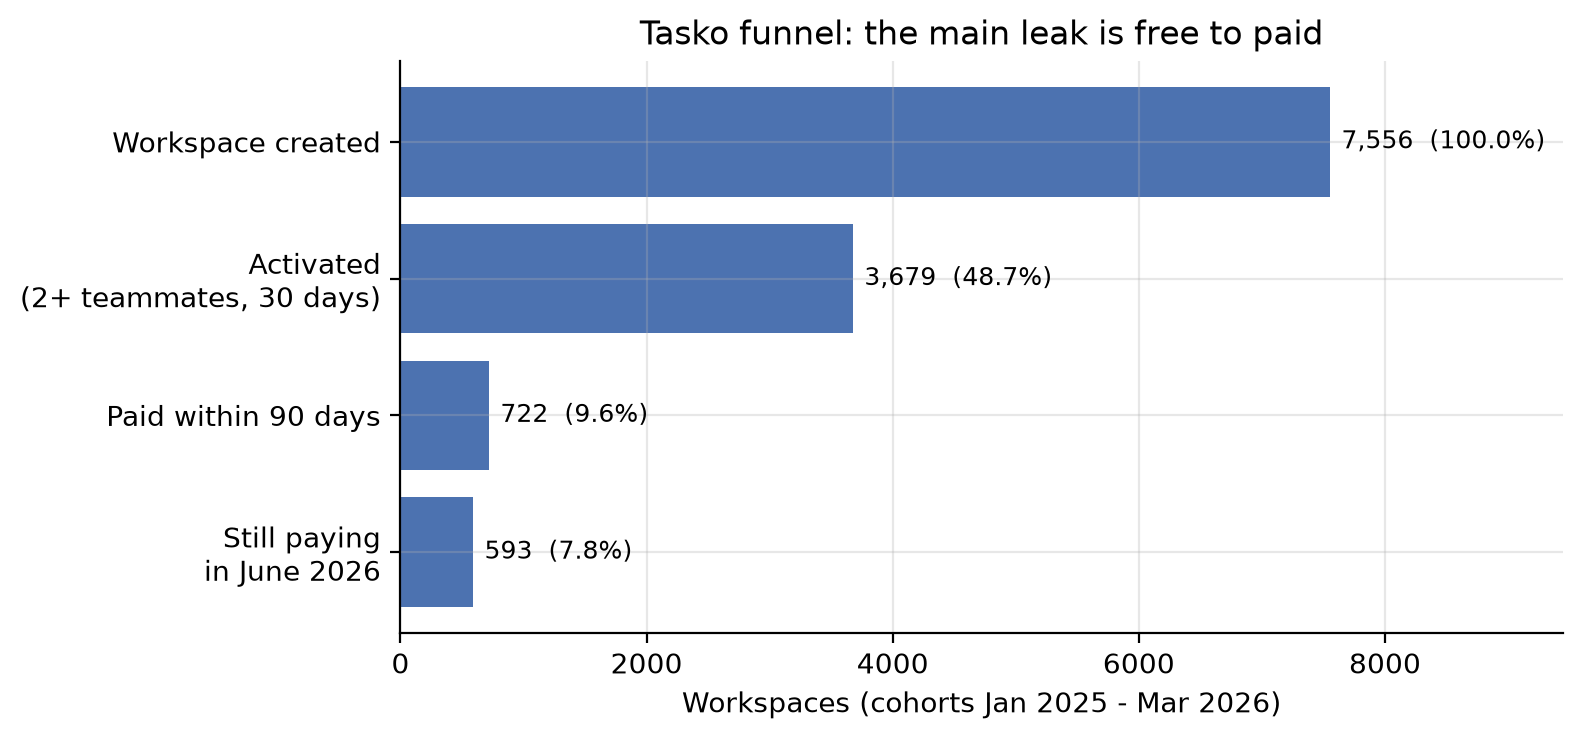
\includegraphics[width=\linewidth]{fig02_funnel.png}
    \end{column}
    \begin{column}{0.46\textwidth}\centering
      \figtitle{Aha moment: conversion jumps at $2+$ teammates}
      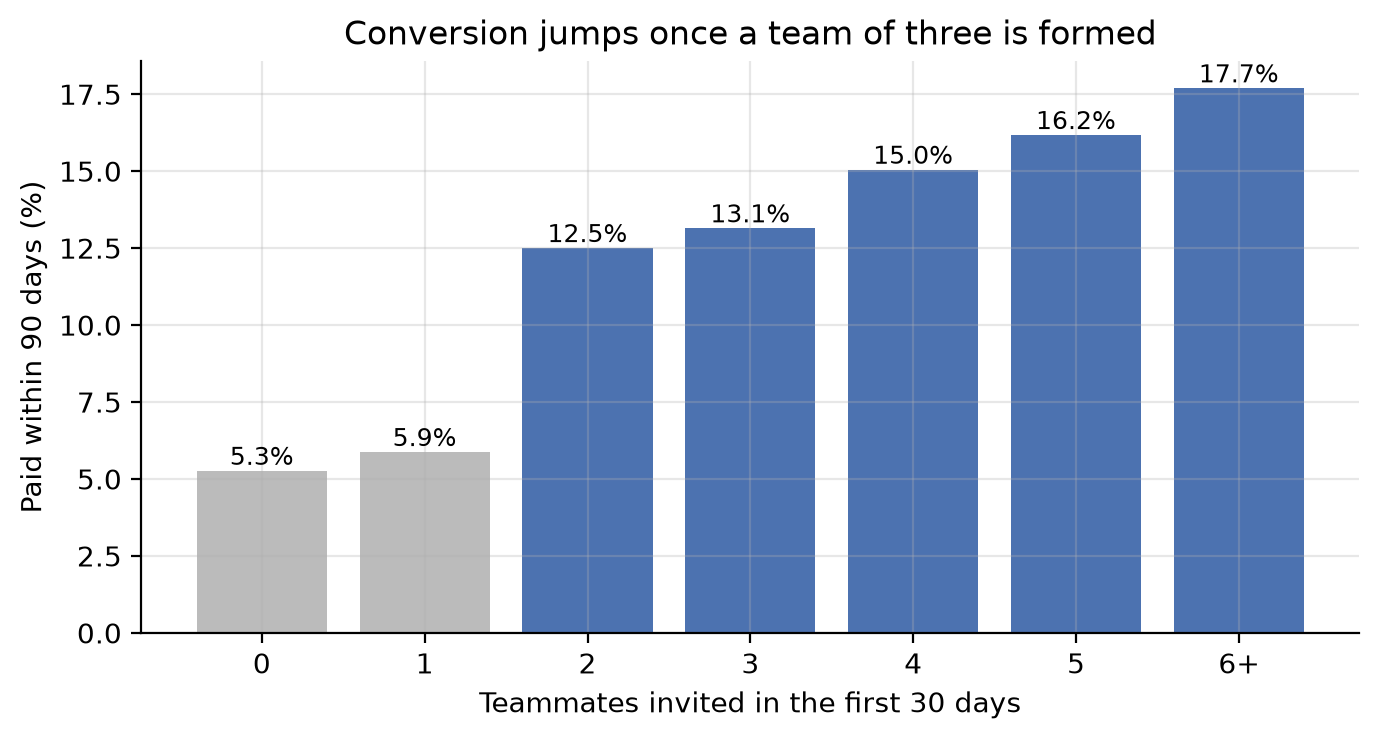
\includegraphics[width=\linewidth]{fig01_aha_moment.png}
    \end{column}
  \end{columns}
  \takeaway{Activated workspaces (48.7\pc{} of sign-ups) convert at \textbf{13.8\pc{} vs 5.6\pc{}} and generate \textbf{70\pc{} of all paying customers}. Once paying, 82\pc{} stay.}
\end{frame}

% ==================================================================
% SLIDE 4: THE GROWTH LOOP
% ==================================================================
\begin{frame}{A real guest loop that compounds with the base, but $K \ll 1$}
  \begin{columns}[T]
    \begin{column}{0.48\textwidth}\centering
      \figtitle{New workspaces per month by channel}
      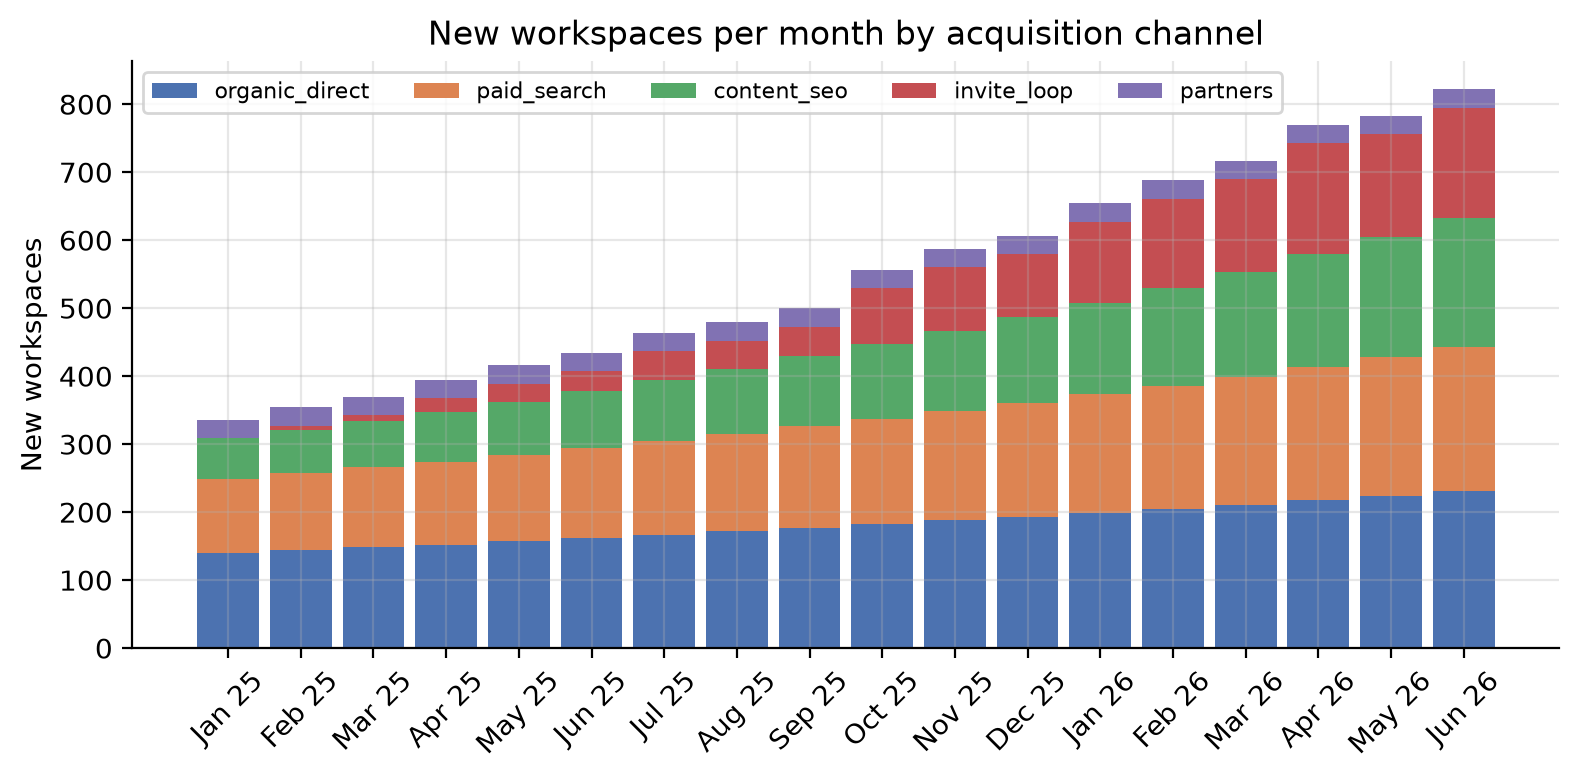
\includegraphics[width=\linewidth]{fig03_new_workspaces.png}
    \end{column}
    \begin{column}{0.50\textwidth}\centering
      \figtitle{Monthly loop rate \& 180-day effective $K$-factor}
      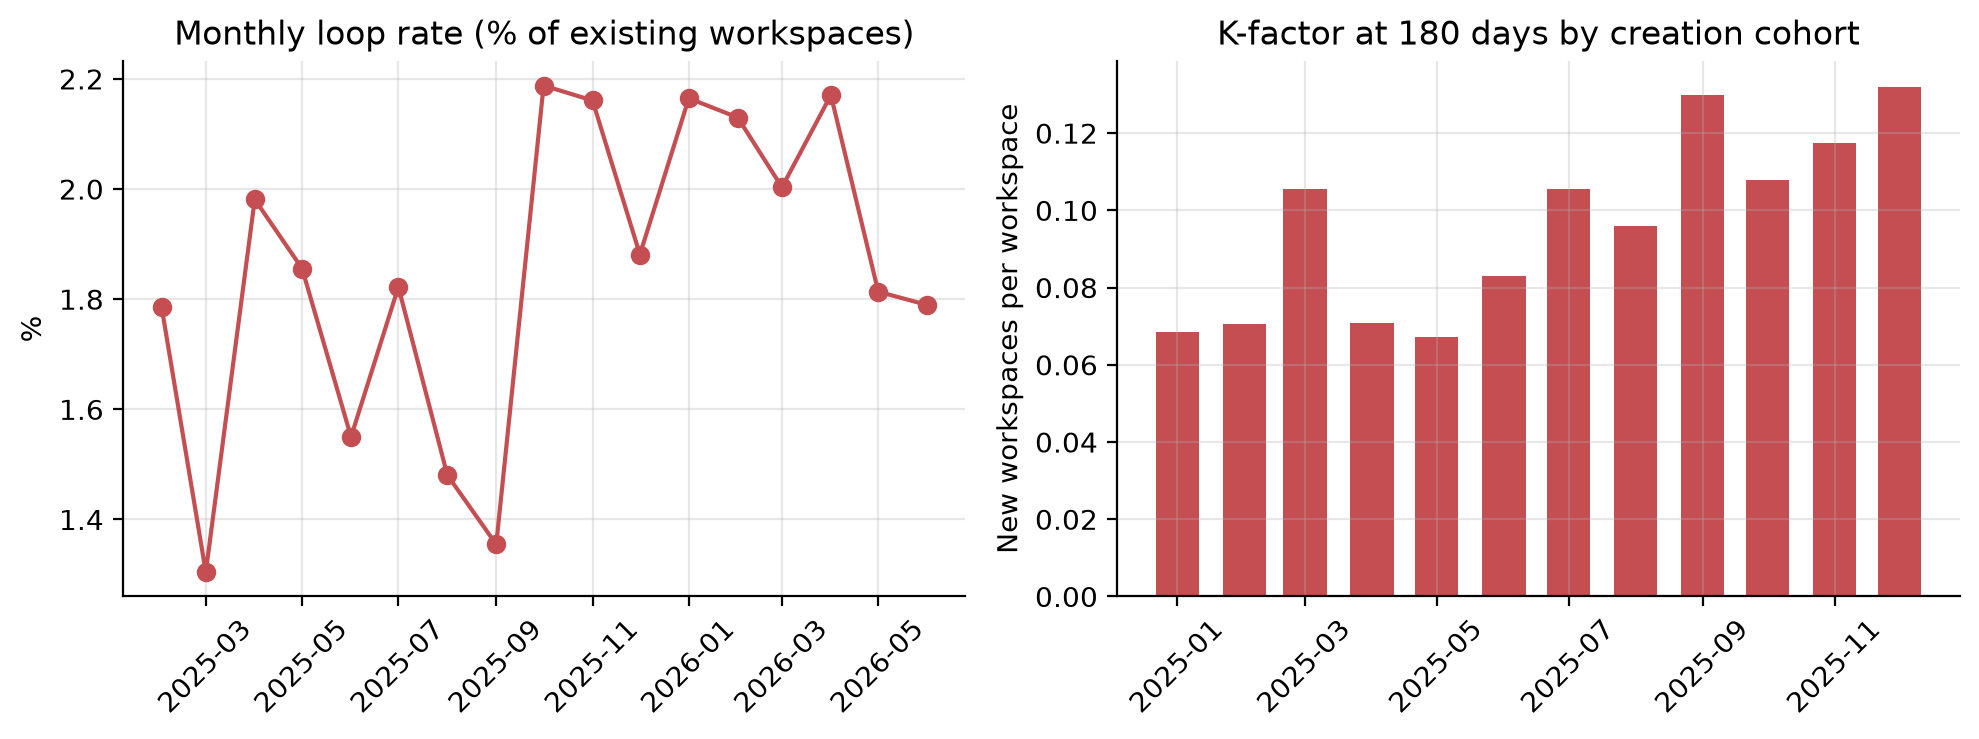
\includegraphics[width=\linewidth]{fig04_invite_loop.png}
    \end{column}
  \end{columns}
  \takeaway{\texttt{invite\_loop} rises from \textbf{0\pc{} to 19.8\pc{}} of acquisition. With $K_{180\text{d}}$ rising from \textbf{0.09 to 0.12} (median lag 146 days), the loop multiplies acquisition rather than replacing it, fed by the total stock of workspaces, independently of activation or channel.}
\end{frame}


% ==================================================================
% SLIDE 5: CHANNELS & LIKE-FOR-LIKE
% ==================================================================

\begin{frame}{Paid search converts less, even like for like}
  \begin{columns}[T]
    \begin{column}{0.52\textwidth}\centering
      \figtitle{Raw channel performance: activation, conversion, ARPA}
      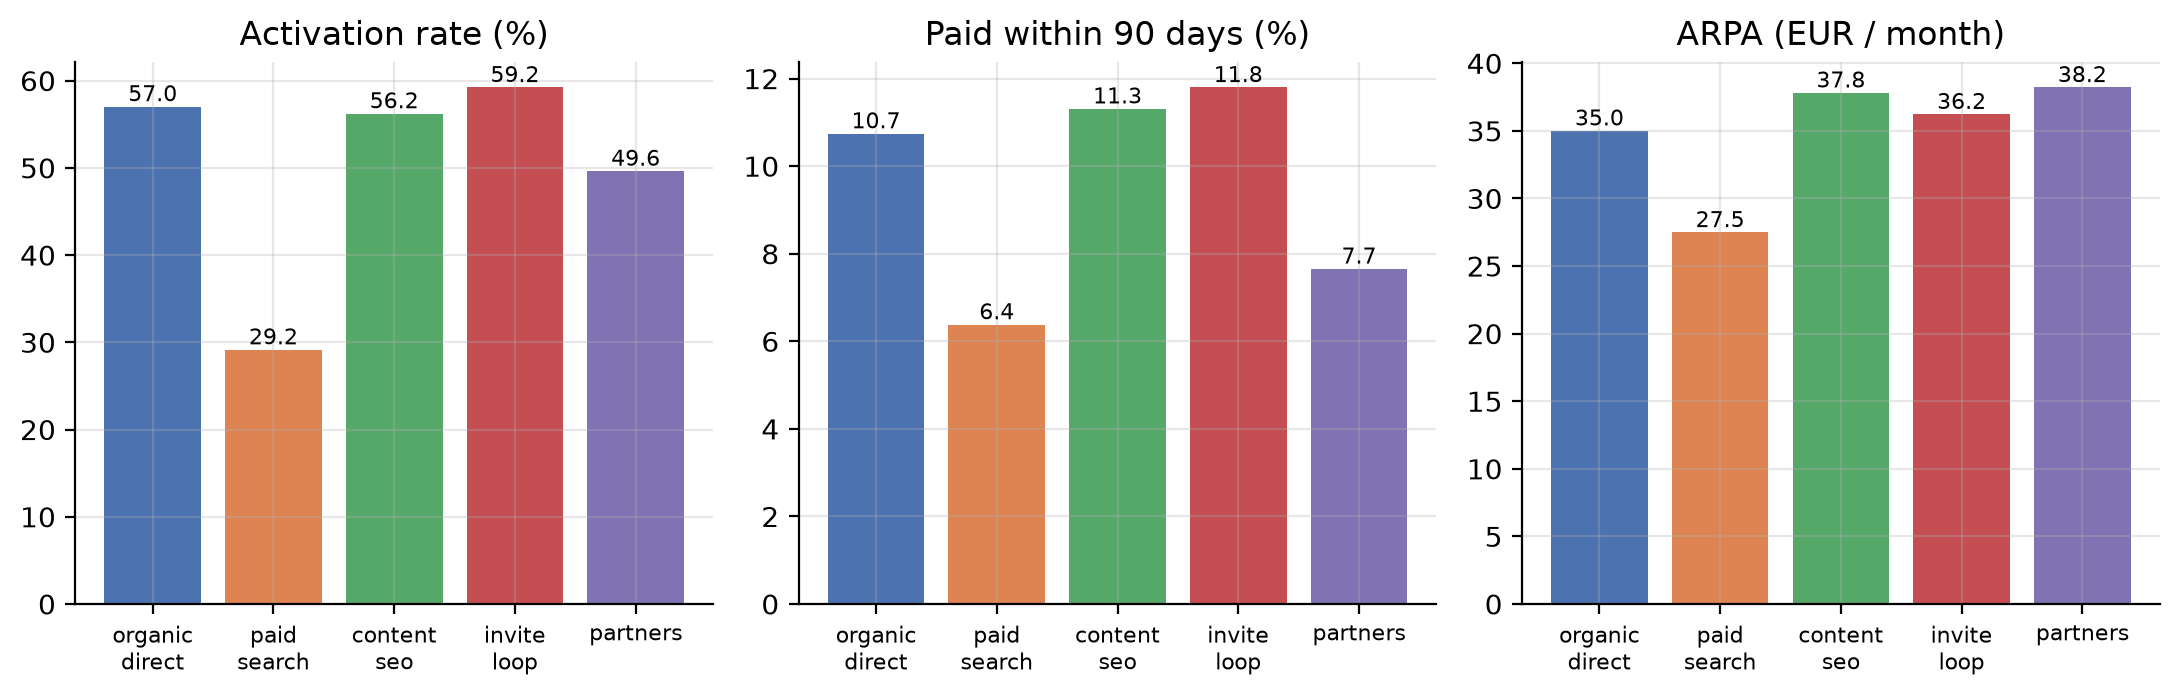
\includegraphics[width=\linewidth]{fig05_channel_kpis.png}
    \end{column}
    \begin{column}{0.46\textwidth}\centering
      \figtitle{90-day conversion (\%) within size \& activation}
      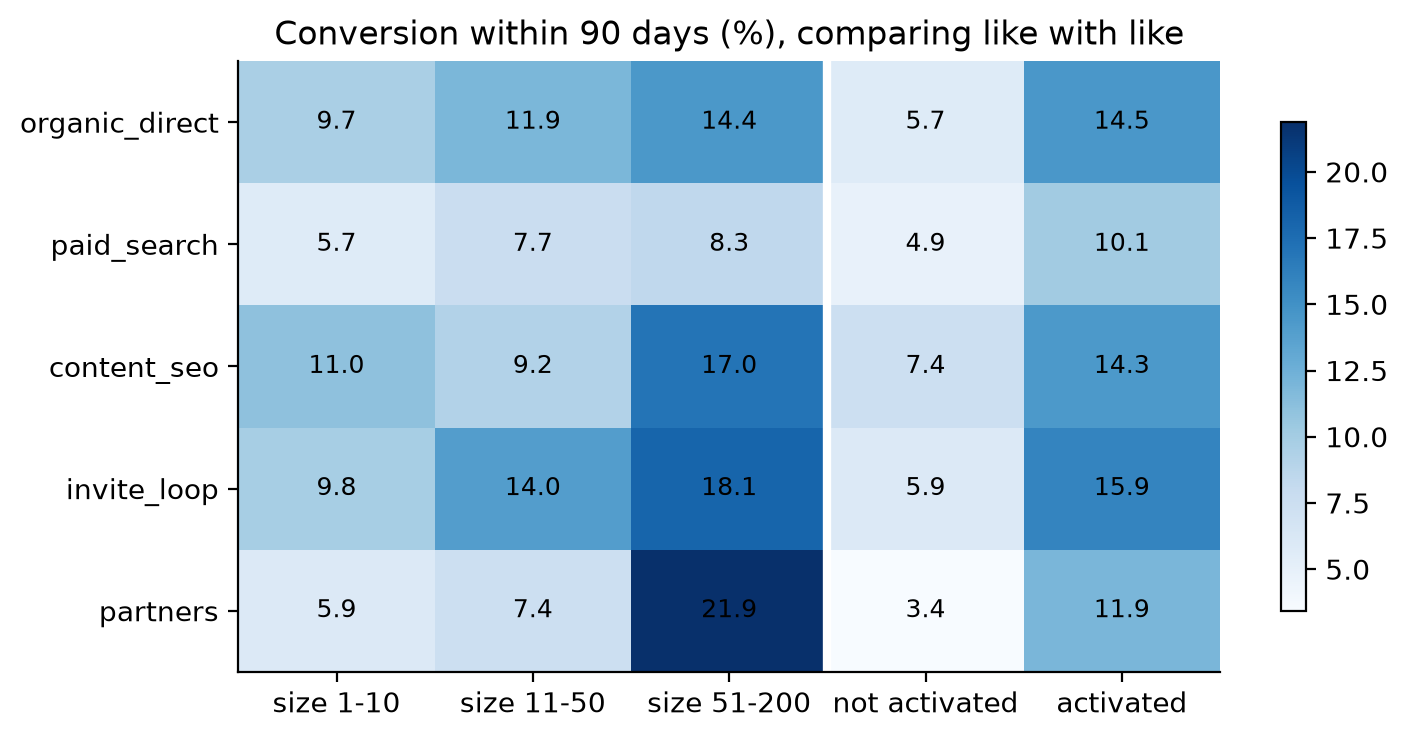
\includegraphics[width=\linewidth]{fig06_like_for_like.png}
    \end{column}
  \end{columns}
  \takeaway{Same size mix across channels ($60/29/9\pc{}$), yet \textbf{among activated teams} paid search converts at \textbf{10.1\pc{} vs 14.3--15.9\pc{}}. Its one edge is \textbf{retention} (lowest churn, 2.7\pc{}). Segment driver: 51--200 companies bring \textbf{66\eur{} ARPA \& 1.2\pc{} churn} (vs 21\eur{} \& 4.4\pc{}).}
\end{frame}

% ==================================================================
% SLIDE 6: UNIT ECONOMICS
% ==================================================================


\begin{frame}{Unit economics: similar LTV, but paid search costs 2.4$\times$ more per payer}
  \begin{columns}[T]
    \begin{column}{0.49\textwidth}\centering
      \figtitle{CAC vs revenue LTV and LTV\,:\,CAC ratio}
      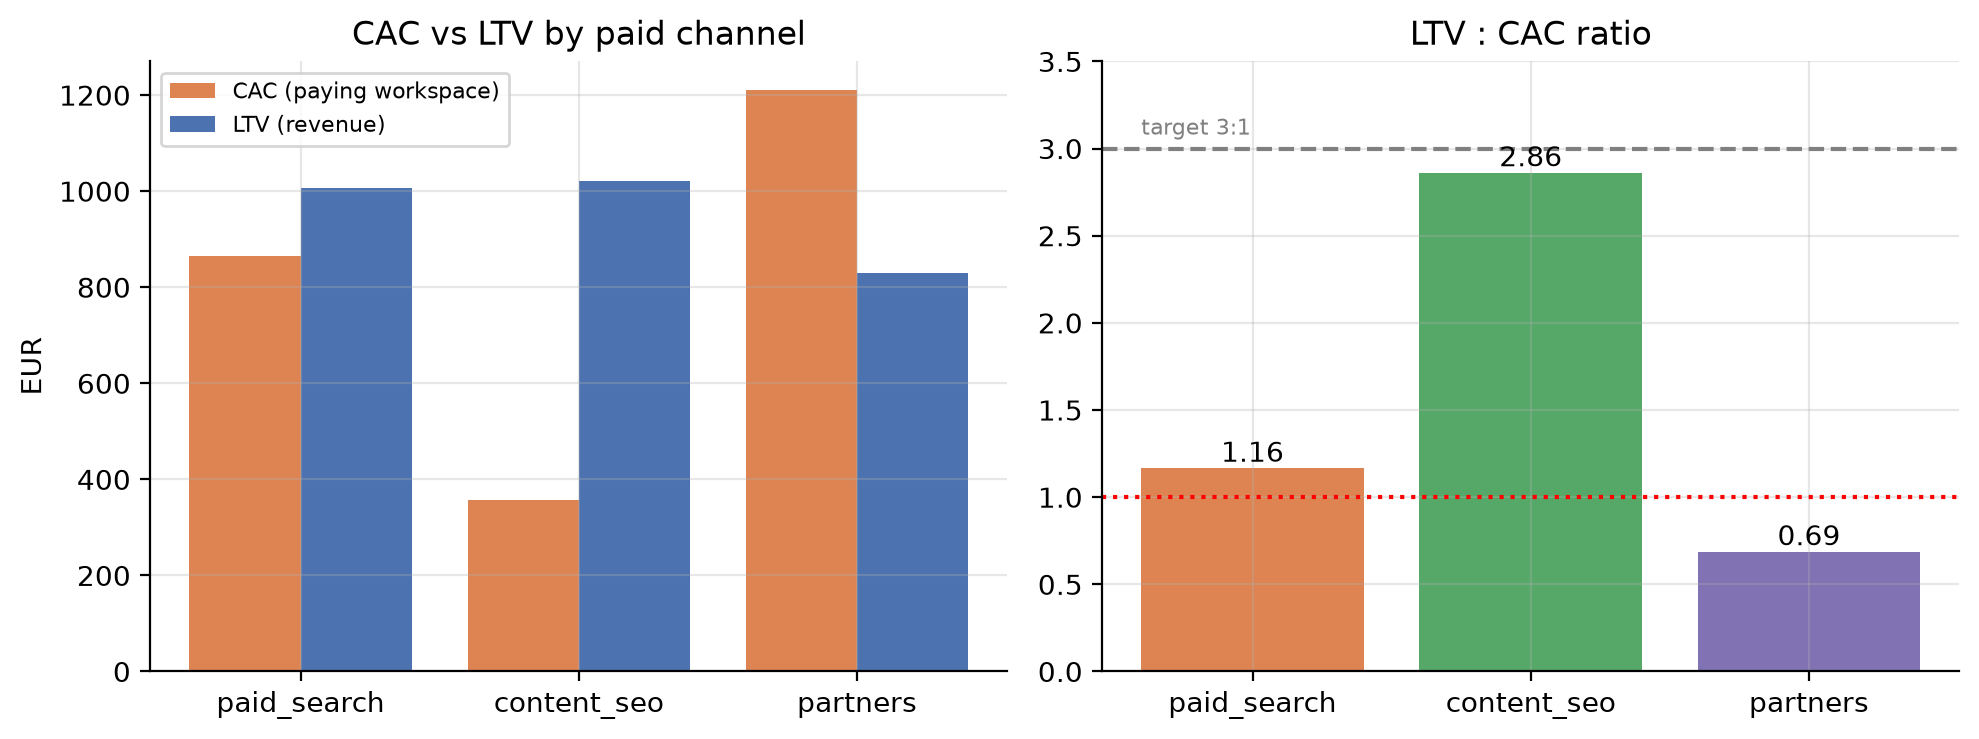
\includegraphics[width=\linewidth]{fig07_unit_economics.png}
    \end{column}
    \begin{column}{0.49\textwidth}\centering
      \figtitle{Monthly spend and cost per sign-up (CPS)}
      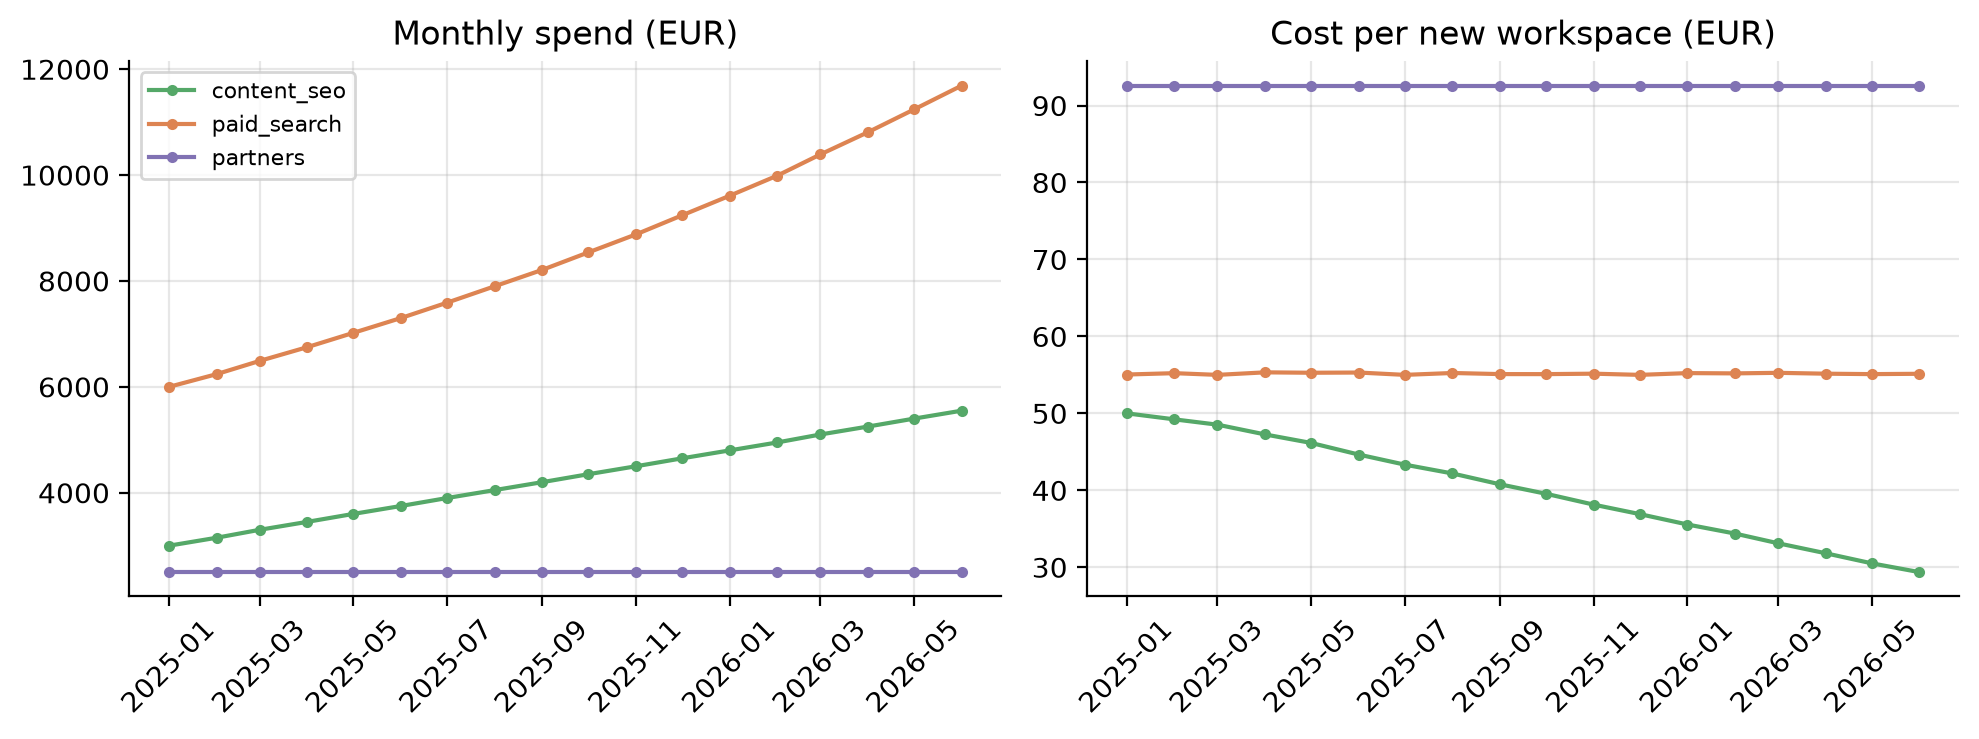
\includegraphics[width=\linewidth]{fig08_spend_and_cost_per_signup.png}
    \end{column}
  \end{columns}
  \vspace{-2pt}
  \centering\scriptsize
  \begin{tabular}{lrrrrrr}
    \toprule
    \textbf{Paid Channel} & \textbf{CPS} & \textbf{Paying CAC} & \textbf{ARPA} & \textbf{Monthly Churn} & \textbf{Revenue LTV} & \textbf{LTV\,:\,CAC / Payback} \\
    \midrule
    \textbf{Content SEO} & 40\eur{} ($50\rightarrow 29$\eur) & 357\eur & 37.8\eur & 3.7\pc & 1,022\eur & \textbf{\color{okgreen}2.86 \;/\; 9.5 months} \\
    \textbf{Paid search} & 55\eur{} (flat, spend $\times 1.95$) & 864\eur & 27.5\eur & 2.7\pc & 1,007\eur & \textbf{\color{accent}1.16 \;/\; 31.5 months} \\
    \textbf{Partners}    & 93\eur{} (flat 27 sign-ups/m) & 1,210\eur & 38.2\eur & 4.6\pc & 830\eur & \textbf{\color{accent}0.69 \;/\; 31.7 months} \\
    \bottomrule
  \end{tabular}
  \vspace{4pt}
  \takeaway{Paid search retains best (2.7\pc{} churn), so its LTV (1,007\eur) matches \\ Content SEO's: the whole gap comes from \textbf{CAC (864\eur{} vs 357\eur)}.}
\end{frame}

% ==================================================================
% SLIDE 7: WHAT CHANGED IN SEPTEMBER 2025
% ==================================================================

\begin{frame}{Mid-September 2025: the onboarding step change}
  \begin{columns}[T]
    \begin{column}{0.47\textwidth}\centering
      \figtitle{First-week invitations jump from 1.1 to 1.9}
      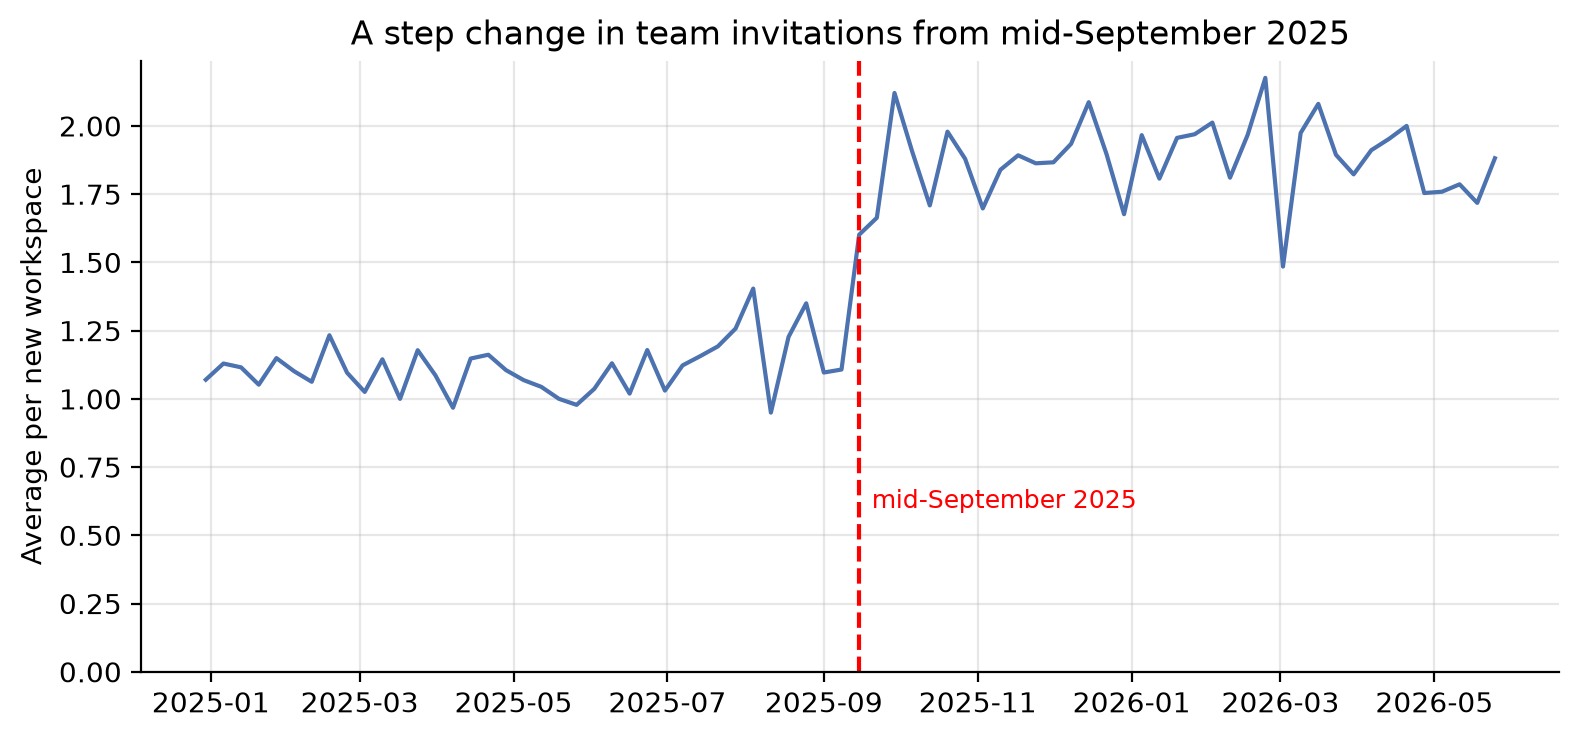
\includegraphics[width=\linewidth]{fig11_change_detection.png}
    \end{column}
    \begin{column}{0.51\textwidth}\centering
      \figtitle{Activation \& conversion before vs after 15 Sep 2025}
      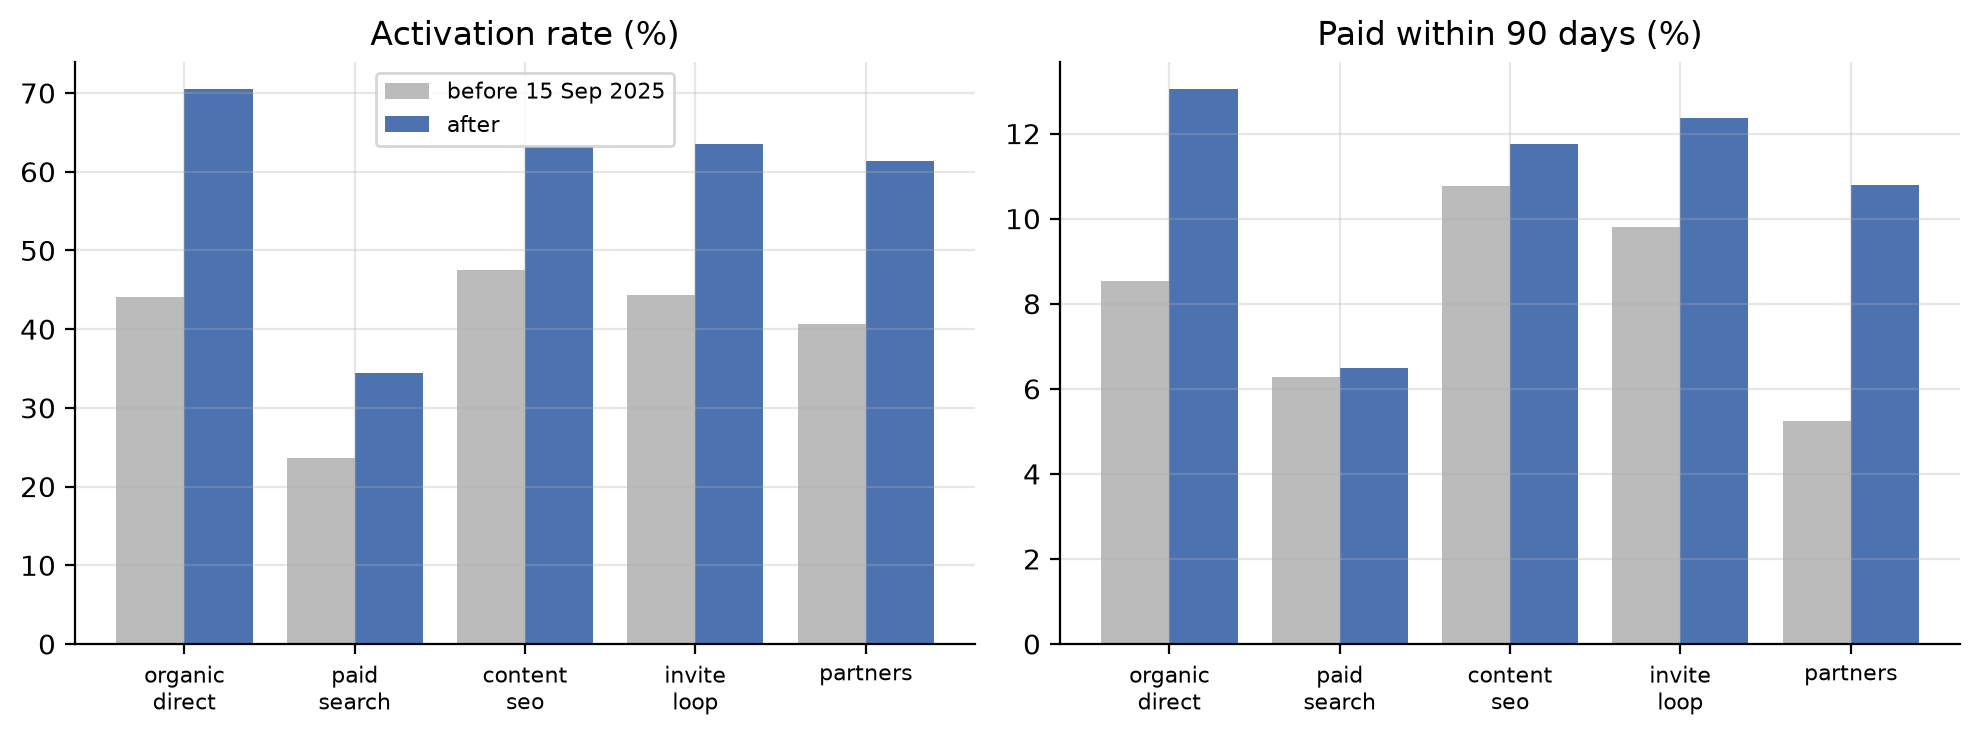
\includegraphics[width=\linewidth]{fig12_before_after.png}
    \end{column}
  \end{columns}
  \takeaway{Permanent product shift: \textbf{loop $K_{180\text{d}}$ $0.086 \rightarrow 0.123$} (whole stock, not activation-specific), with \textbf{churn unchanged} (3.2\pc{} vs 3.3\pc{}). Exception: \textbf{paid search conversion stayed flat} ($6.3\pc{} \rightarrow 6.5\pc{}$).}
\end{frame}

% ==================================================================
% SLIDE 8: GROWTH MODEL & BACKTEST
% ==================================================================
\begin{frame}{Backtest: the model reveals where the business changed}
  \centering
  \figtitle{Out-of-sample backtest: calibrated up to 31 Dec 2025, simulated on Jan -- Jun 2026}
  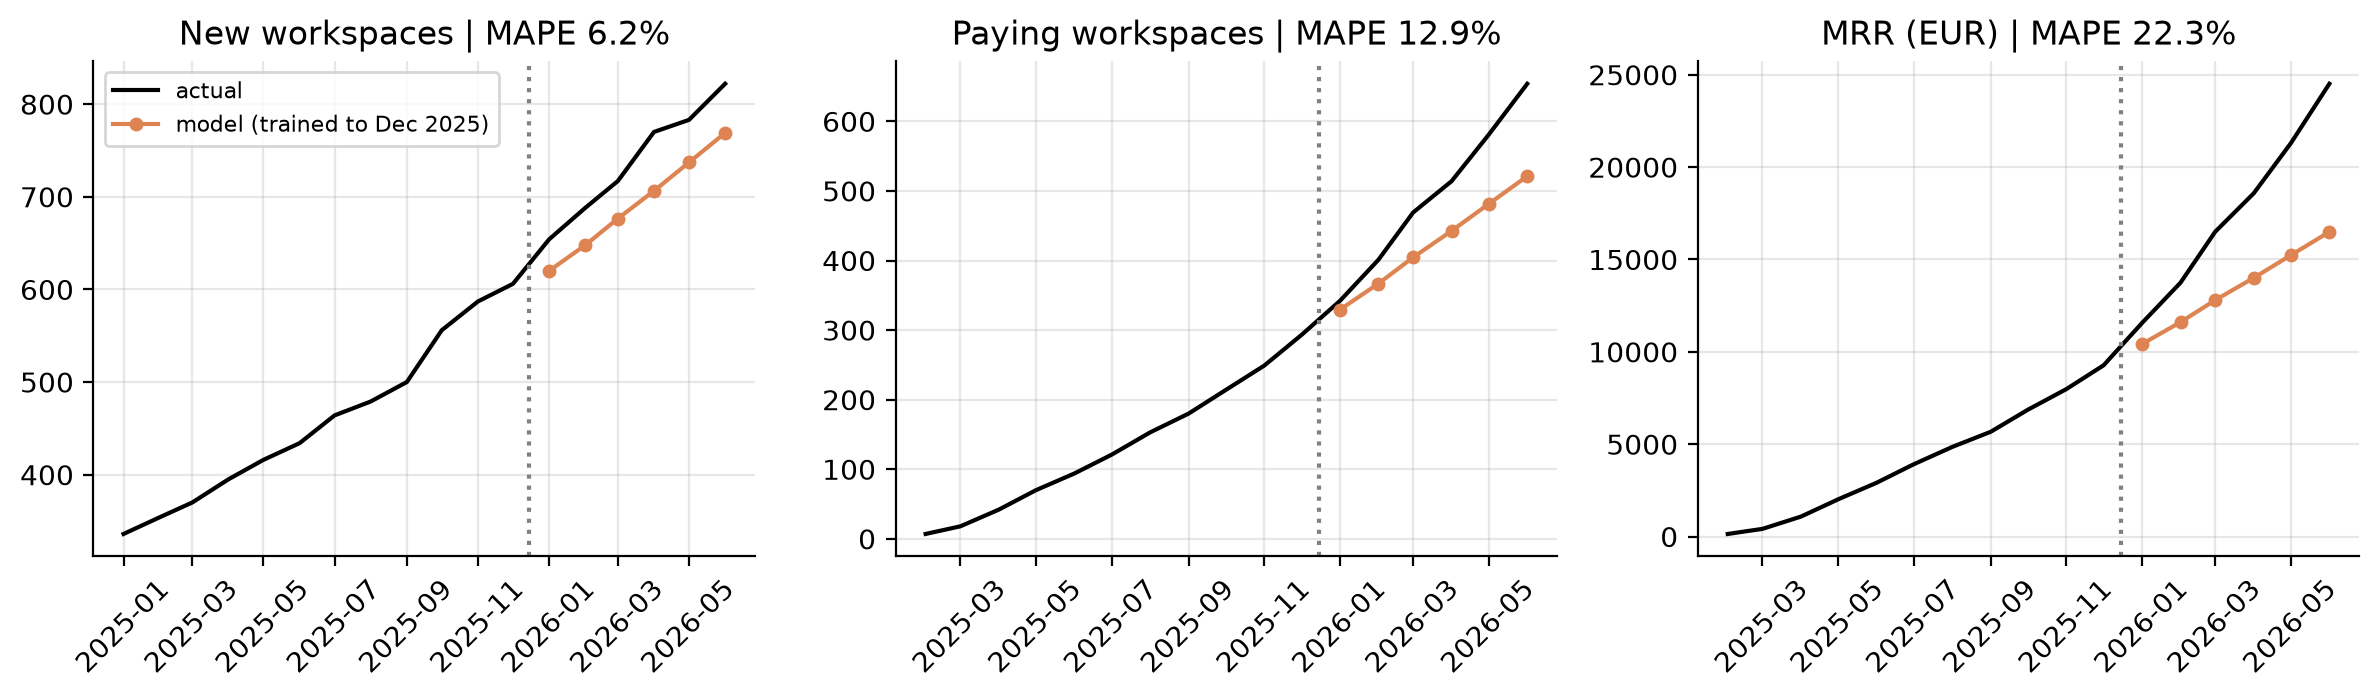
\includegraphics[width=0.95\textwidth]{fig14_backtest.png}
  \vspace{2pt}
  \begin{columns}[T]
    \begin{column}{0.48\textwidth}
      \begin{tcolorbox}[colback=navylight,colframe=navy!50,boxrule=0.4pt,arc=2pt,left=5pt,right=5pt,top=2pt,bottom=2pt]
        \scriptsize\textbf{\color{navy}Model structure:} $\text{New WS}_t = \sum \frac{\text{Spend}_{c,t}}{\text{CPS}_c} + \text{Org}_t + r_{\text{loop}}\text{Stock}_{t-1}$\\
        1--4 month billing lag $\rightarrow$ $\text{Paying}_t$ (churn decay) $\rightarrow$ $\text{MRR}_t = \text{Paying}_t \times \text{ARPA}_t$.
      \end{tcolorbox}
    \end{column}
    \begin{column}{0.48\textwidth}
      \begin{tcolorbox}[colback=accentlight,colframe=accent!60,boxrule=0.4pt,arc=2pt,left=5pt,right=5pt,top=2pt,bottom=2pt]
        \scriptsize\textbf{\color{accent}Error decomposition:} In Dec 2025, Sep cohorts were just turning mature.\\
        + Post-change conversion: Paying MAPE \textbf{12.9\pc{} $\rightarrow$ 4.0\pc{}}.\\
        + Observed H1 2026 ARPA: MRR MAPE \textbf{22.3\pc{} $\rightarrow$ 6.2\pc{}}.
      \end{tcolorbox}
    \end{column}
  \end{columns}
\end{frame}

% ==================================================================
% SLIDE 9: SCENARIOS & SENSITIVITY
% ==================================================================
\begin{frame}{June 2027 projections (42 to 109\,k\eur{} MRR): post-signup levers dominate}
  \begin{columns}[T]
    \begin{column}{0.50\textwidth}\centering
      \figtitle{Three empirical scenarios (Jul 2026 -- Jun 2027)}
      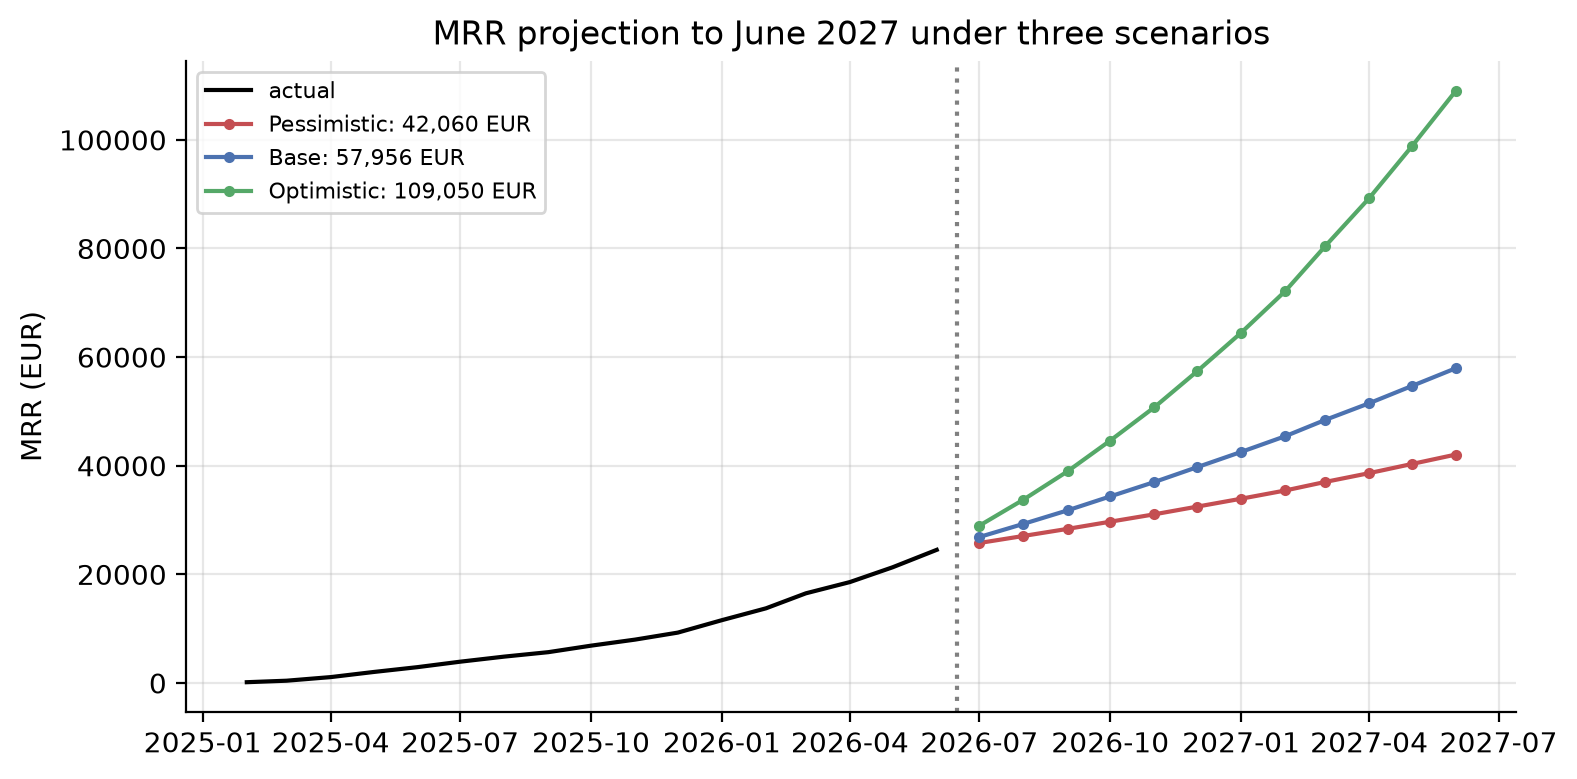
\includegraphics[width=\linewidth]{fig15_scenarios.png}
    \end{column}
    \begin{column}{0.48\textwidth}\centering
      \figtitle{Sensitivity of June 2027 MRR to $\pm 20\pc{}$ lever shifts}
      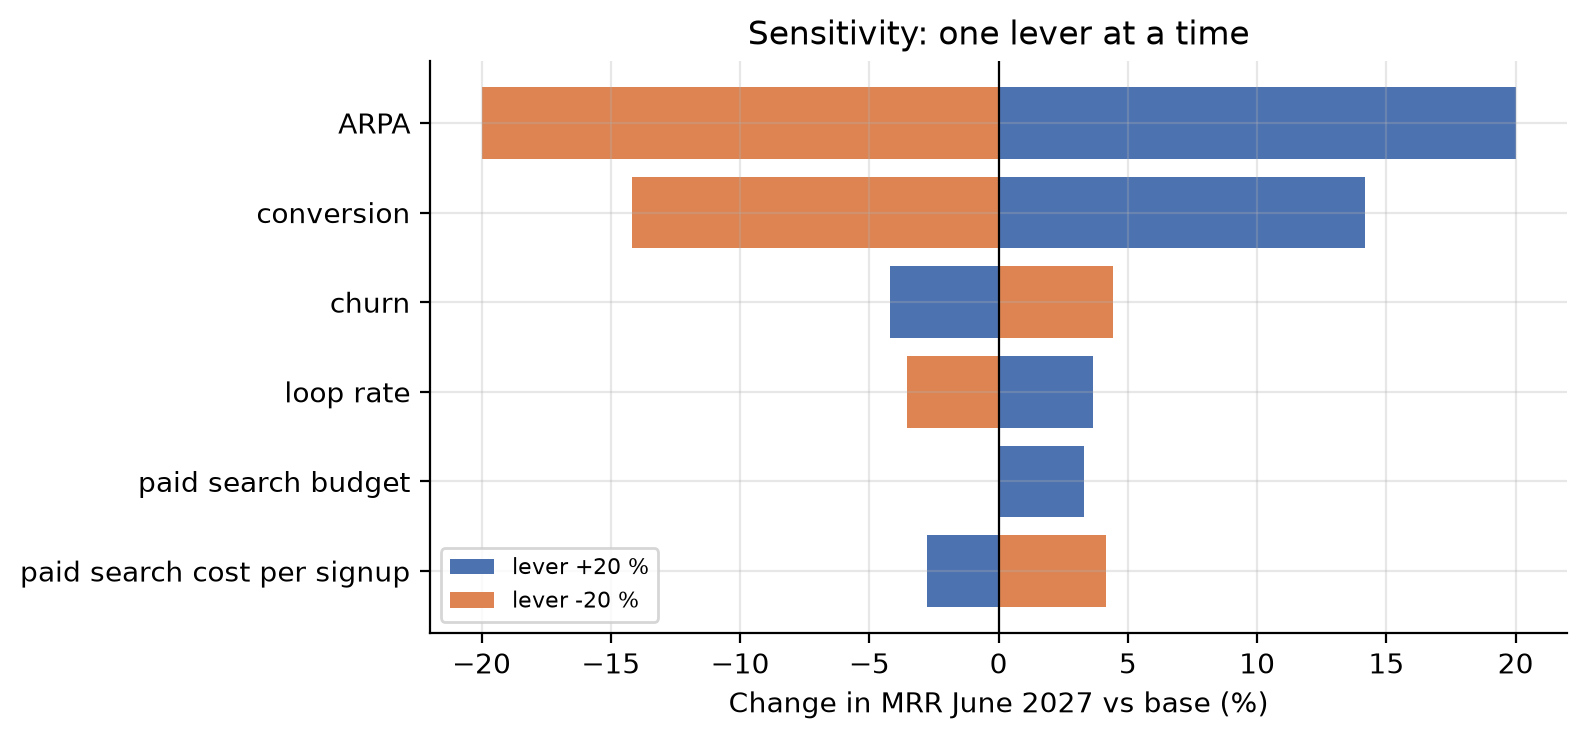
\includegraphics[width=\linewidth]{fig16_sensitivity.png}
    \end{column}
  \end{columns}
  \takeaway{New workspaces barely differ across scenarios (12.5\,k to 13.5\,k). Lifting \textbf{ARPA (+20\pc{})} or \textbf{conversion (+14.2\pc{})} drives massive MRR gains, whereas \textbf{+20\pc{} paid search budget adds only +3.3\pc{} MRR}.}
\end{frame}

% ==================================================================
% SLIDE 10: NORTH STAR METRIC, A/B TEST & RECOMMENDATIONS
% ==================================================================

\begin{frame}{North Star Metric, A/B test plan \& strategic roadmap}
  \vspace{-3pt}
  \begin{columns}[T]
    \begin{column}{0.45\textwidth}\centering
      \figtitle{NSM: Workspaces reaching a team of 3 / month}
      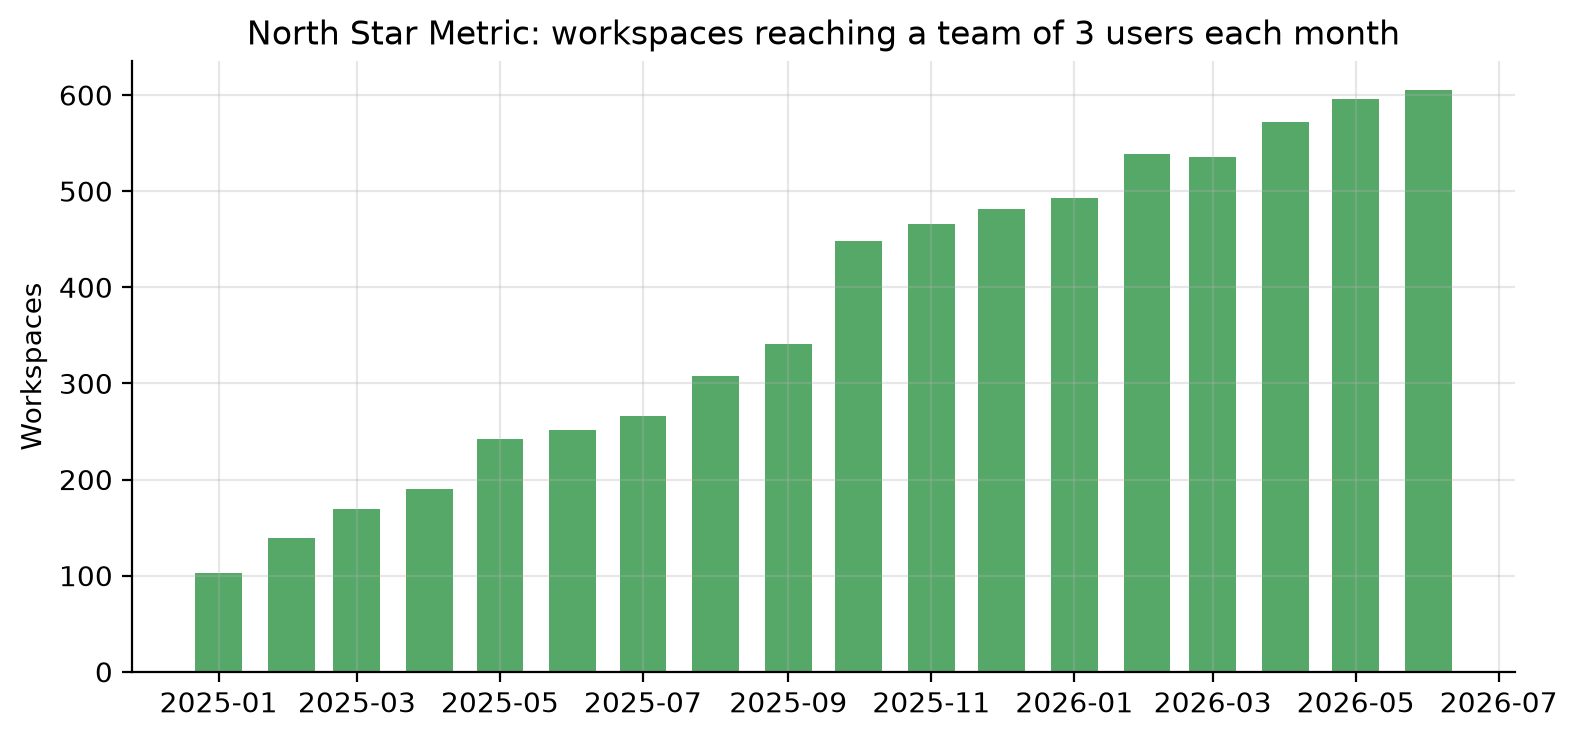
\includegraphics[width=0.92\linewidth]{fig13_north_star.png}
      \vspace{-5pt}
      \begin{tcolorbox}[colback=oklight,colframe=okgreen,boxrule=0.5pt,arc=2pt,left=4pt,right=4pt,top=2pt,bottom=2pt]
        \scriptsize\color{darkgray}\textbf{\color{okgreen}Why this NSM (605/m in Jun 2026):} captures team value, predicts conversion ($\times 2.5$) \& ARPA, less sensitive to paid search volume.
        \textbf{Guardrails:} 90d conversion \& churn.
      \end{tcolorbox}
    \end{column}
    \begin{column}{0.52\textwidth}
      \begin{tcolorbox}[colback=white,colframe=navy,boxrule=0.5pt,arc=2pt,left=4pt,right=4pt,top=1pt,bottom=1pt,boxsep=1pt,title={\scriptsize\bfseries A/B Test: Fixing Paid Search Onboarding}]
        \scriptsize
        \begin{itemize}\setlength{\itemsep}{0pt}\setlength{\parskip}{0pt}
          \item \textbf{Treatment:} Optional \emph{``Invite 2 teammates''} step before 1st project (50/50 split on \texttt{paid\_search}, no dark patterns).
          \item \textbf{Metrics:} Primary = 30d activation (34.5\pc{}); Secondary = 90d conversion (6.5\pc{}).
          \item \textbf{Sizing ($\alpha=5\pc{}$, power $80\pc{}$):} \textbf{+8 pts MDE} $\rightarrow$ \textbf{577/arm} ($\approx$ \textbf{5.7 months}).
        \end{itemize}
      \end{tcolorbox}
      \vspace{-4pt}
      \begin{tcolorbox}[colback=navylight,colframe=navy,boxrule=0.5pt,arc=2pt,left=4pt,right=4pt,top=1pt,bottom=1pt,boxsep=1pt,title={\scriptsize\bfseries 4 Recommendations before Series A}]
        \scriptsize
        \begin{enumerate}\setlength{\itemsep}{0pt}\setlength{\parskip}{0pt}
          \item \textbf{Steer on the Team of 3 NSM} across product \& marketing.
          \item \textbf{Cap paid search} until A/B test proves conversion; \textbf{shift growth to Content SEO} (LTV\,:\,CAC 2.86, 9.5m payback).
          \item \textbf{Stop or renegotiate Partners} (LTV\,:\,CAC 0.69) per activated team.
          \item \textbf{Prioritise seat expansion \& Business plan} (1.2--2.1\pc{} churn, 66\eur{} ARPA).
        \end{enumerate}
      \end{tcolorbox}
    \end{column}
  \end{columns}
\end{frame}

\end{document}
